% File: algo.tex
% Date: Wed Jun 17 21:41:53 2015 +0800
% Author: Yuxin Wu <ppwwyyxxc@gmail.com>

%File: feature.tex
%Author: Yuxin Wu <ppwwyyxx@gmail.com>

\section{Feature Detection and Matching}
Lowe's SIFT algorithm\cite{sift} is implemented in \verb|feature/*.cc|.
The procedure of the algorithm and some results are briefly described as followed.
\begin{enumerate}
  \item \textbf{Scale Space} (\verb|feature/dog.cc|)

    A Scale Space consisting of $ S \times O$ grey images is built.
    The original image is resized in $ O$ different sizes (AKA. octaves), and each is then Gaussian-Blured
    by $ S$ different $ \sigma$.
    \begin{figure}[H]
      \centering
      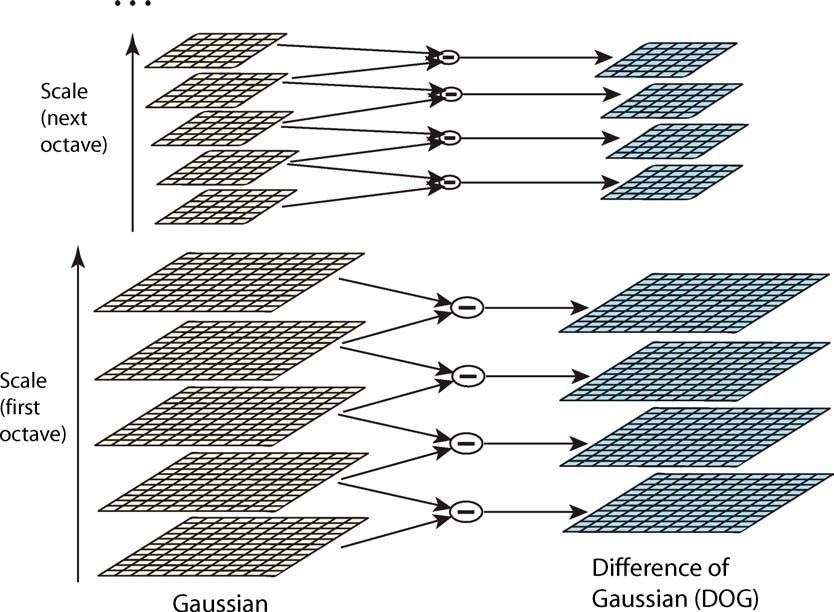
\includegraphics[scale=0.35]{res/dog.jpg}
      \caption{Scale Space and DOG Space \label{fig:dog}}
    \end{figure}

    Feature is detected on different resized version of the original
    image, to ensure scale invariant.

    The gaussian blur here is implemented by applying two 1-D convolutions, rather than
    a 2-D convolution. This speeds up the computation significantly.

  \item \textbf{DOG Space}(\verb|feature/dog.cc|)

    In each octave, calculate the differences of every two adjacent blured images, to build a Difference-of-Gaussian Space.
    Therefore, DOG Space consists of $ (S - 1) \times O$ grey images.
    As shown in \figref{dog}.

  \item \textbf{Extrema Detection}(\verb|feature/extrema.cc|)

    In DOG Space, detect all the minimum and maximum
    by comparing a pixel with its 26 neighbors in \textbf{three directions}: $ x, y, \sigma$.
    See \figref{extrema} and \figref{extrema2}
    \begin{figure}[H]
      \begin{minipage}[b]{0.46\linewidth}
        \centering
        \includegraphics[scale=0.4]{res/extrema.png}
        \caption{Extrema Detection\label{fig:extrema}}
      \end{minipage}
      \hspace{1em}
      \begin{minipage}[b]{0.46\linewidth}
        \centering
        \includegraphics[scale=0.35]{res/extrema_lenna.png}
        \caption{Extrema Example\label{fig:extrema2}}
      \end{minipage}
    \end{figure}

  \item \textbf{Keypoint Localization}(\verb|feature/extrema.cc|)

    Use \textbf{parabolic interpolation} to look for the accurate location of the extrema.
    Then reject the points with \textbf{low contrast}(by thresholding pixel value)
    or \textbf{on the edge}(by thresholding principle curvature), to get more distinctive features.
    See \figref{feature1}, \figref{feature2}, \figref{feature3}.
    \begin{figure}[H]
      \begin{minipage}[b]{0.46\linewidth}
        \centering
        \includegraphics[scale=0.4]{res/feature_after_offset.png}
        \caption{After Localization \label{fig:feature1}}
      \end{minipage}
      \hspace{1em}
      \begin{minipage}[b]{0.46\linewidth}
        \centering
        \includegraphics[scale=0.4]{res/feature_after_contrast.png}
        \caption{After Rejecting Low Contrast\label{fig:feature2}}
      \end{minipage}
    \end{figure}

  \item \textbf{Orientation Assignment}(\verb|feature/orientation.cc|)
    \label{sec:orientation_assign}

    First, we calculate \textbf{gradient and orientation} for every point in the Scale Space.
    For each keypoint detected by the previous procedure,
    the orientations of its nearby points will be collected and used to build an \textbf{orientation histogram},
    weighted by the magnitude of the gradient at each point, together with a gaussian kernel centered at the keypoint.
    The peak in the histogram is chosen to be the major orientation of the keypoint, as shown by the arrows in \figref{feature4}.

    \begin{figure}
      \begin{minipage}[b]{0.46\linewidth}
        \centering
        \includegraphics[scale=0.4]{res/feature_point.png}
        \caption{After Eliminating Edge Point\label{fig:feature3}}
      \end{minipage}
      \hspace{1em}
      \begin{minipage}[b]{0.46\linewidth}
        \centering
        \includegraphics[scale=0.4]{res/feature_dir.png}
        \caption{After Assigning Orientation\label{fig:feature4}}
      \end{minipage}
    \end{figure}

  \item \textbf{Descriptor Representation}(\verb|feature/sift.cc|)

    D. Lowe suggested choosing 16 points around the keypoint, to build orientation histograms for each point, similar
    to the method in \secref{orientation_assign}.
    Each histogram uses 8 different possible values(bins). Therefore the final SIFT feature is a \textbf{128-dimensional}
    floating point vector.
    Since the major orientation of the keypoint is known, by using relative orientation to the keypoint,
    this feature is roatation-invariant.

  \item \textbf{Feature Matching}(\verb|feature/{feature,match}.cc|)

    \textbf{Euclidean distance} of the 128-dimensional descriptor is the criteria for feature matching between two images.
    A match is considered not convincing and therefore rejected,
    if the distances from it to its closest neighbor and second-closest neighbor are similar.
    A result is shown in \figref{match}.
    \begin{figure}[H]
      \centering
      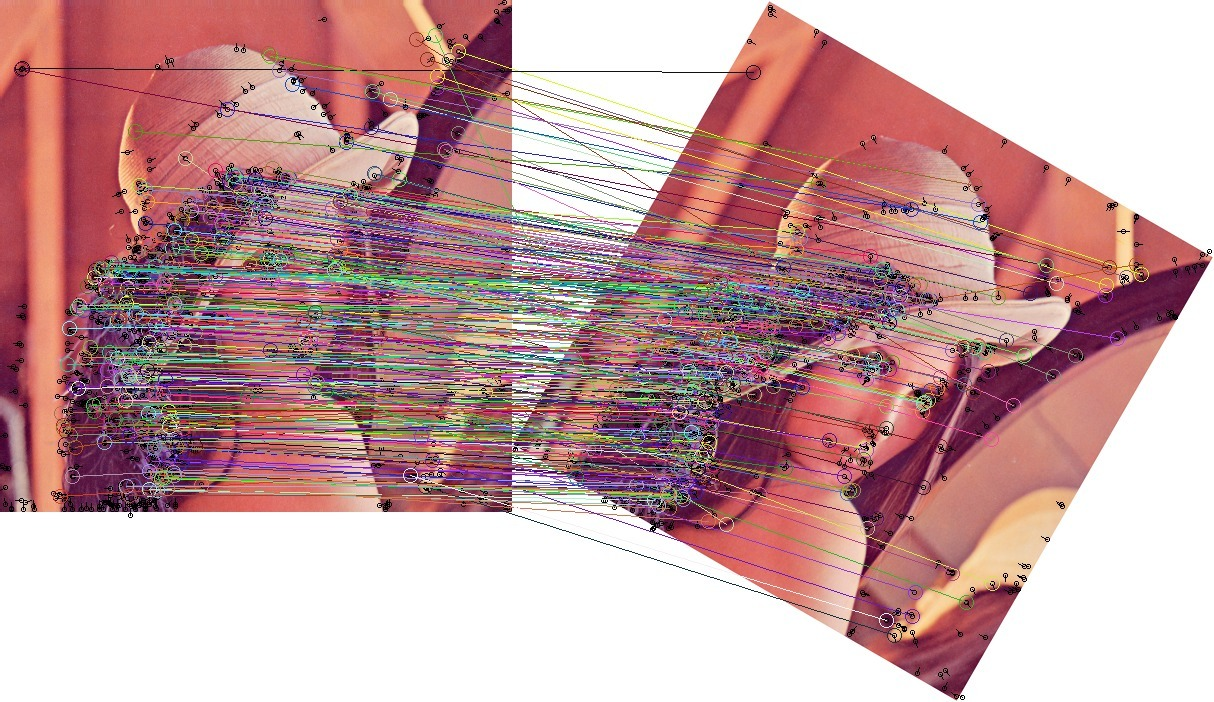
\includegraphics[width=\textwidth]{res/match.jpg}
      \caption{Matching Result\label{fig:match}}
    \end{figure}

    I use FLANN library \cite{flann} to query 2-nearest-neighbor among feature vectors.
    To calculate Euclidean distance of two vectors, Intel SSE3 intrinsics are used to speed up.

\end{enumerate}


%File: transform.tex
%Author: Yuxin Wu <ppwwyyxx@gmail.com>

\section{Transformation}
\label{sec:transform}

For any two images taken from a camera at some fixed point,
they can be related by a homography matrix $H$,
such that for a pair of corresponding point $ p=(x,y,1), q = (u,v,1)$,
we have
\[ p \sim Hq\]
The homogrpahy matrix has the following two fomulations:
\begin{enumerate}
  \item Homography I: $H = \begin{bmatrix} a_{11} &a_{12} & a_{13}\\ a_{21} & a_{22} & a_{23}\\ a_{31} & a_{32} & 1\end{bmatrix}$

  \item Homography II:
    $H = \begin{bmatrix} a_{11} &a_{12} & a_{13}\\ a_{21} & a_{22} & a_{23}\\ a_{31} & a_{32} & a_{33}\end{bmatrix} $
    and $\begin{Vmatrix} H \end{Vmatrix} = 1$
\end{enumerate}

When two images are taken with only camera translation
and rotation aligned with the image plane (no skew),
then they can be related by an affine matrix of the following form:
\[ A = \begin{bmatrix} a_{11} &a_{12} & a_{13}\\ a_{21} & a_{22} & a_{23}\\ 0 & 0 & 1\end{bmatrix} \]


\textbf{RANSAC} (Random Sample Consensus) algorithm\cite{ransac} is used to calculate a transformation matrix.
In every iteration, several matched pairs is randomly chosen to calculate a best-fit transformation matrix,
and the pairs which agree with the matrix are taken as inliers. It's implemented in \verb|stitch/transform_estimate.cc|.

Given a set of matches, affine and the first kind of homography transformation can be solved
by least-squares fitting an over-determined linear system.
The second kind of homography transformation can be solved by finding eigenvectors.
These estimation methods are implemented in \verb|lib/imgproc.cc|.

After each matrix estimation, I performed
a ``health check`` to the matrix,
to avoid mal-formed transformation
estimated from false matches.
This includes two checks: (see \verb|stitch/homography.hh|)
\begin{enumerate}

  \item  The skew factor in homography
    ($ H_{3,1},H_{3,2}$) cannot be too large. Their
    absolute values are usually less than 0.002.

  \item Flipping cannot happen in image stitching.
    A homography is rejected if it flips either $x$
    or $y$ coordinate.
\end{enumerate}

% TODO overlap test
For a matched pair of images,
a confidence for this match
is assigned by taking the ratio of inliers
among all the feature matches. This is
suggested by \cite{panoramic-sift}, and is useful
in the construction of global structure.

%File: cylinder.tex
%Author: Yuxin Wu <ppwwyyxx@gmail.com>

\section{Cylinder Mode}
\label{sec:cylinder}
\subsection{Necessity of Projection}
If a rotational input is given, as most panoramas are built,
using planar homography leads to \textbf{vertical distortion}, such as \figref{distort}.
\begin{figure}[H]
  \centering
  \includegraphics[width=0.9\textwidth]{res/distort.png}
  \caption{Vertical Distortion with Homography on a Planar\label{fig:distort}}
\end{figure}

This is because a panorama is essentially an image taken with
a cylindrical or spherical lens, not a planar lens any more.
Under this circumstance, a circle around the camera (in \figref{distort}) should
become a line.

There are two ways to handle with this problem: to warp before or after
transform estimation.
\footnote{A good app revealing the reason of this projection can be seen at \url{http://graphics.stanford.edu/courses/cs178-12/applets/projection.html}}
These are the two modes used in this system. In this section we will
introduce the algorithms used in cylinder mode.

\subsection{Warp}
One way of doing this is to project each image
to a cylinder surface at the beginning, by the following formula:

\[  \begin{cases}
    x' = \arctan{\dfrac{x-x_c}{f}}\\
    y' = \dfrac{y-y_c}{\sqrt{(x-x_c)^2 + f^2}}
  \end{cases}\]
where $ f$ is the focal length of the camera, and $ x_c, y_c$ is the center of image.
See \verb|stitch/warp.cc|

After projecting all images to the cylinder surface, images can be
simply stitched together by an affine transformation.
The result is in shown in \figref{cyl}. Note that the white line on
the ground is straightened.
\begin{figure}[H]
  \centering
  \begin{minipage}[b]{0.24\linewidth}
    \includegraphics[scale=0.3]{res/1.png}
  \end{minipage}
  \begin{minipage}[b]{0.24\linewidth}
    \includegraphics[scale=0.3]{res/2.png}
  \end{minipage}
  \begin{minipage}[b]{0.24\linewidth}
    \includegraphics[scale=0.3]{res/3.png}
  \end{minipage}
  \begin{minipage}[b]{0.24\linewidth}
    \includegraphics[scale=0.3]{res/4.png}
  \end{minipage}

  \includegraphics[width=0.9\textwidth]{res/warped_stitch.png}
  \caption{Stitching Result After Projection\label{fig:cyl}}
\end{figure}

\subsection{Straightening}
\begin{figure}[H]
  \centering
  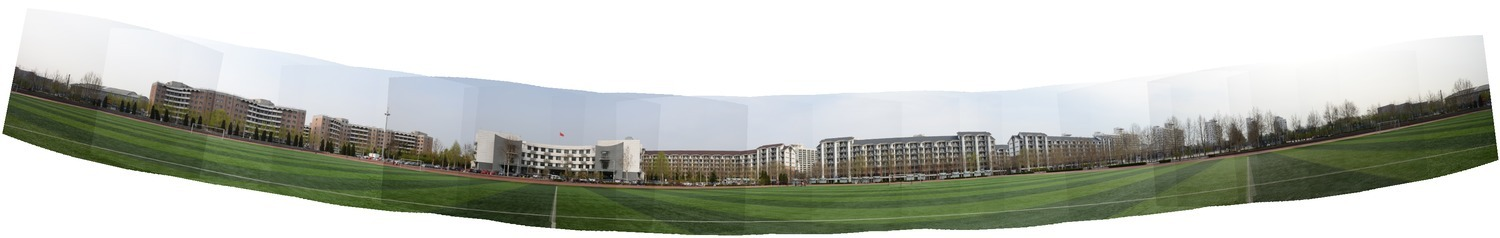
\includegraphics[width=\textwidth]{res/bend.jpg}
  \caption{Bended Panorama\label{fig:bend}}
\end{figure}

Since the tilt angle of camera is unknown,
the projection to the cylinder could still lead to distortion.
Then the output panorama would be bended as shown in \figref{bend}.
Instead of using the first image as the pivot, and calculating all the other transformation relative to it,
using the image in the middle as the pivot can help reduce the tilt effect.
Apart from that, I found a method to reduce the effect, by searching for $ y_c$
in the above warping formula.

Since the effect is caused by camera tilt, $ y_c$ could differ from $ \dfrac{height}{2}$.
The algorithm works by changing $ y_c$ and find a value which leads to the most straight result. See \verb|Stitcher::update_h_factor()|.
After this processes, the result is like \figref{unbend}.

\begin{figure}[H]
  \centering
  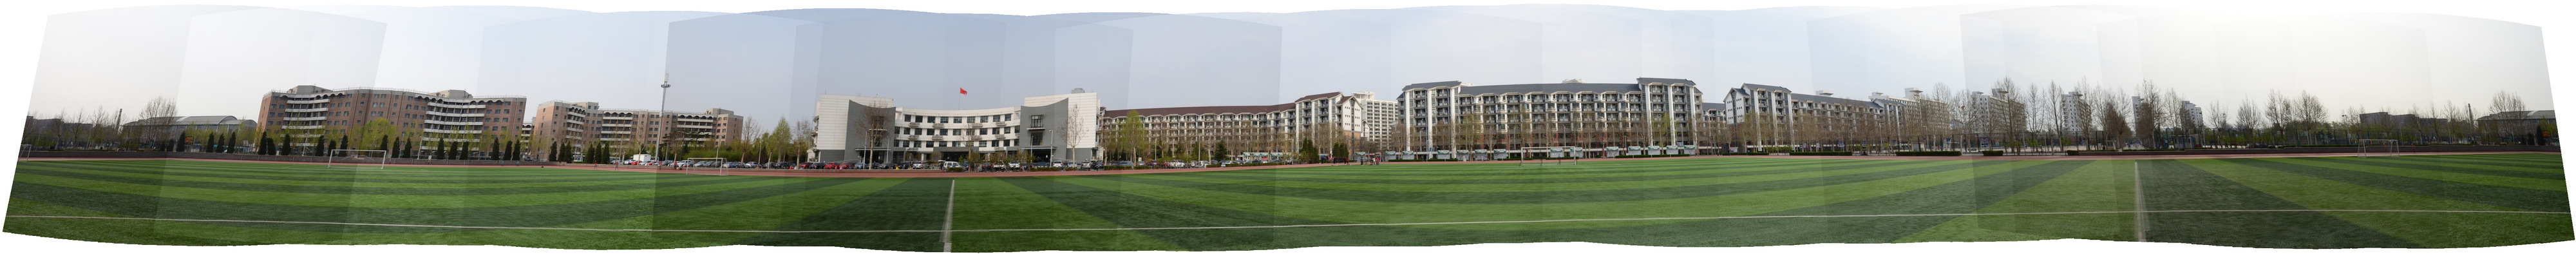
\includegraphics[width=\textwidth]{res/unbend.jpg}
  \caption{After bend correction\label{fig:unbend}}
\end{figure}

The change of $y_c$ is not enough, since we are still warping
images to a vertical cylinder.
The error can be seen at the left and right edges in \figref{unbend}.
To account for this error, I used a perspective transform
to align the left and right edges (\verb|Stitcher::perspective_correction|). The result is in \figref{unbend-persp}
\begin{figure}[H]
  \centering
  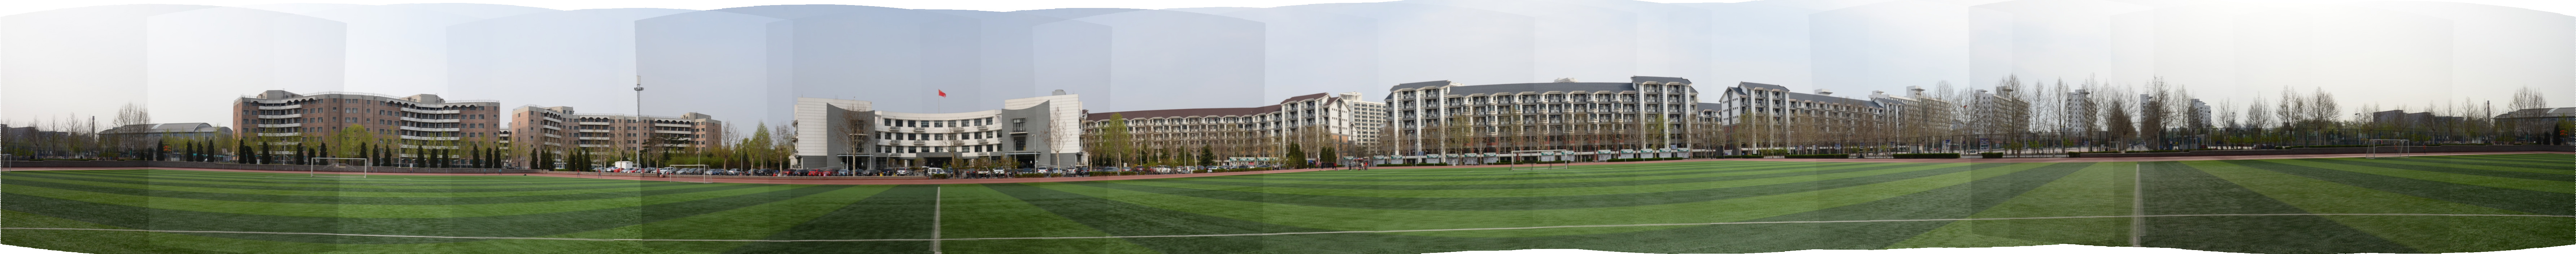
\includegraphics[width=\textwidth]{res/unbend-persp.jpg}
  \caption{After perspective correction \label{fig:unbend-persp}}
\end{figure}


%File: general.tex
%Author: Yuxin Wu <ppwwyyxx@gmail.com>

\section{Camera Estimation Mode}
\label{sec:camera_estimate}
\subsection{Intuition}
The cylinder mode assume a known focal length and pure rotational panorama, to
warp them on cylinder surface at the beginning.
We want to get rid of these assumptions.

One method I tried is to estimate pairwise homographies,
and directly stitch them together. To avoid distortion like \figref{distort},
I performed a cylindrical warp \textbf{after} the transformation.
Then I get something like this:
\begin{figure}[H]
  \centering
  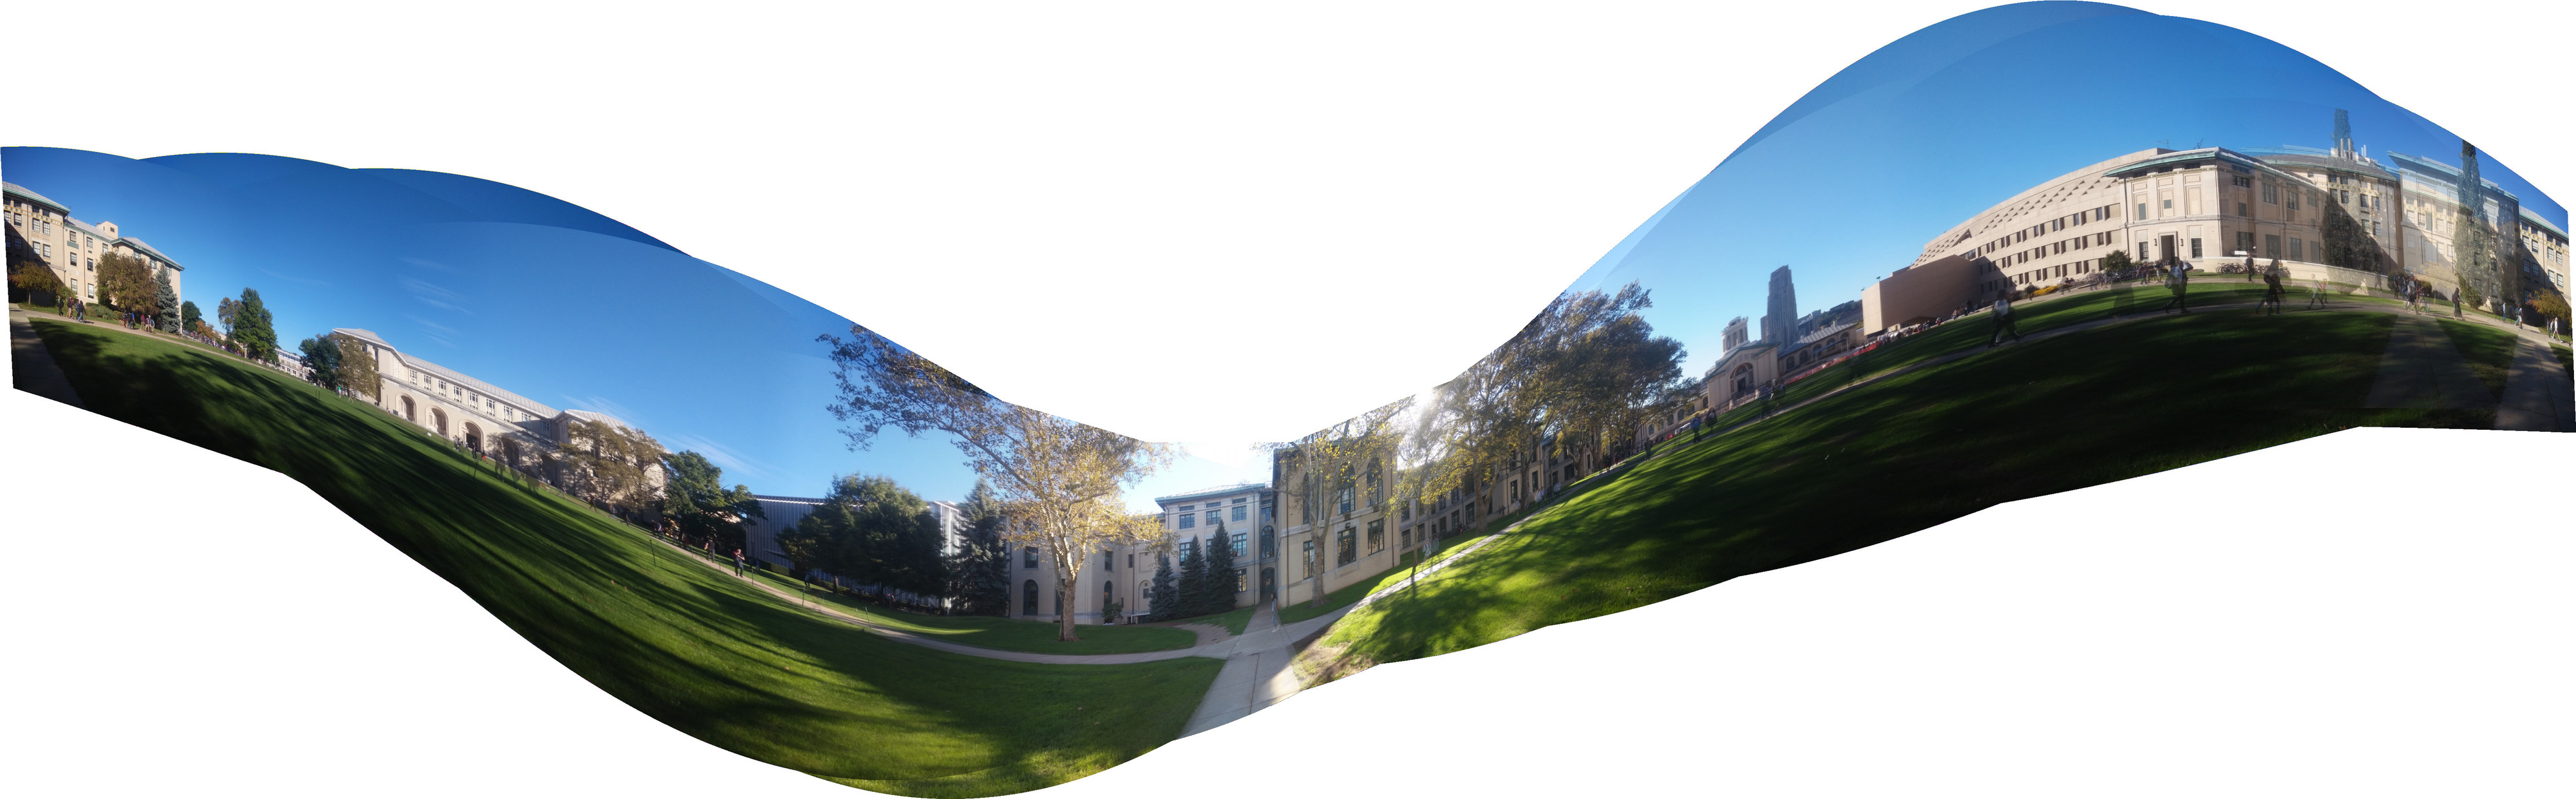
\includegraphics[width=1\textwidth]{res/CMU1-noestimate.jpg}
  \caption{CMU campus, directly stitched and then warped to cylinder}
\end{figure}

This is likely caused by our weak assumption on homography matrix.
A homography is estimated as a 3 by 3 matrix with the only
constraint being the scaling factor. However,
a homography is actually formed as:
\[ H_{1,2} = K_1R_1R_2^{-1}K_2^{-1}\]
where $K,R$ are intrinsic and rotation matrix of each camera.
From this formulation there should be a geometric constrain on each $H$,
which is not built into our initial estimation.
That's why the overall geometric structural is broken, although the matching pairs
are still well overlapped.

To overcome this problem, I estimated initial $K, R$ for each camera, from pairwise homographies.
Then, a global optimization is used to refine the parameters in $K, R$.
Finally, pairwise homographies are rebuilt from our refined $K, R$.

\subsection{Initial Estimation}
As suggested by \cite{focal}, focal length
can be roughly estimated from pairwise homographies. This is implemented in \verb|stitch/camera.cc|.
I used it to produce initial estimation of
focal length and assign it to each camera.

By assuming a rotation matrix for certain pivot image being identical,
other rotation matrices
can be estimated one by one using pairwise homography:
\[ R_1 = K_1^{-1}H_{1,2}K_2R_2\]

To reduce accumulated error,
I first construct a max-spanning tree by using
confidence of pairwise matches calculated in \secref{transform} (\verb|Stitcher::max_spanning_tree()|).
Then each time the most confidence pair is used to estimate
an unknown rotation matrix from a known one.

After obtaining a guess of $K$ and $R$ for each image,
pairwise homographies can be reconstructed and used to
stitch image together. A result is given below. Note that
the distortion is gone due to our constraints on the formulation
of pairwise homographies, but the quality is not satisfactory.
\begin{figure}[H]
  \centering
  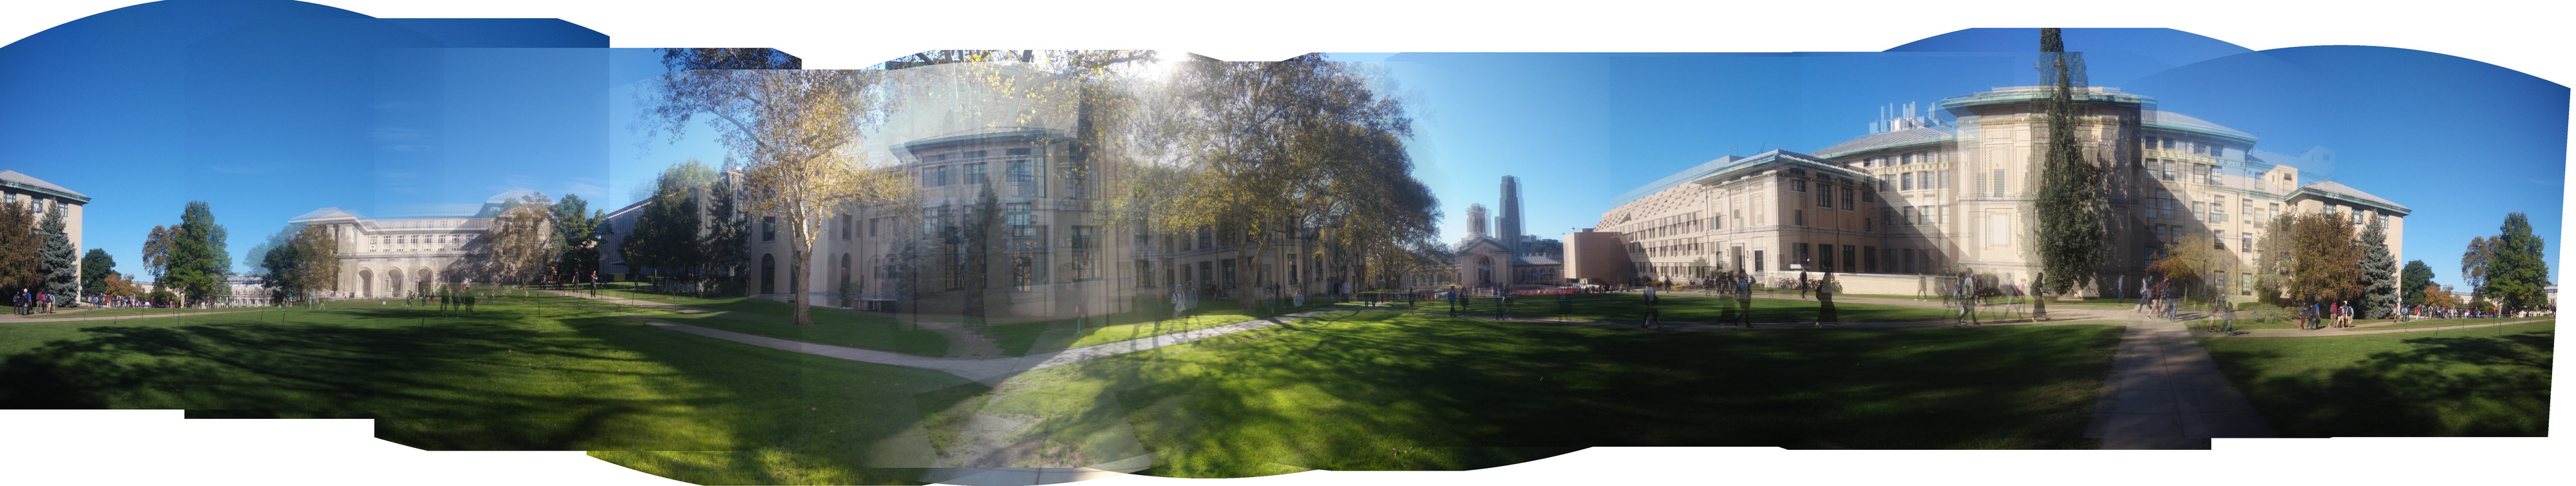
\includegraphics[width=\textwidth]{res/initial_camera.jpg}
  \caption{Initial guess of camera parameters}
\end{figure}

\subsection{Bundle Adjustment}

I implemented bundle adjustment in \verb|stitch/bundle_adjuster.cc|,
to globally optimize all the camera parameters.
The object is to minimize the sum of error of every matching pair of pixels.
The object function can be optimized in Levenberg-Marquardt algorithm
\footnote{\url{https://en.wikipedia.org/wiki/Levenberg–Marquardt_algorithm}}.
For simplicity, I used numerical differentiation to calculate
the Jacobian, although a closed-form formula is available,
as shown in \cite{panoramic-sift}.

During the optimization, the best params so far is kept.
The optimization ended when the error doesn't decrease
in the last 5 iterations.

After the optimization, the above panorama looks much better:
\begin{figure}[H]
  \centering
  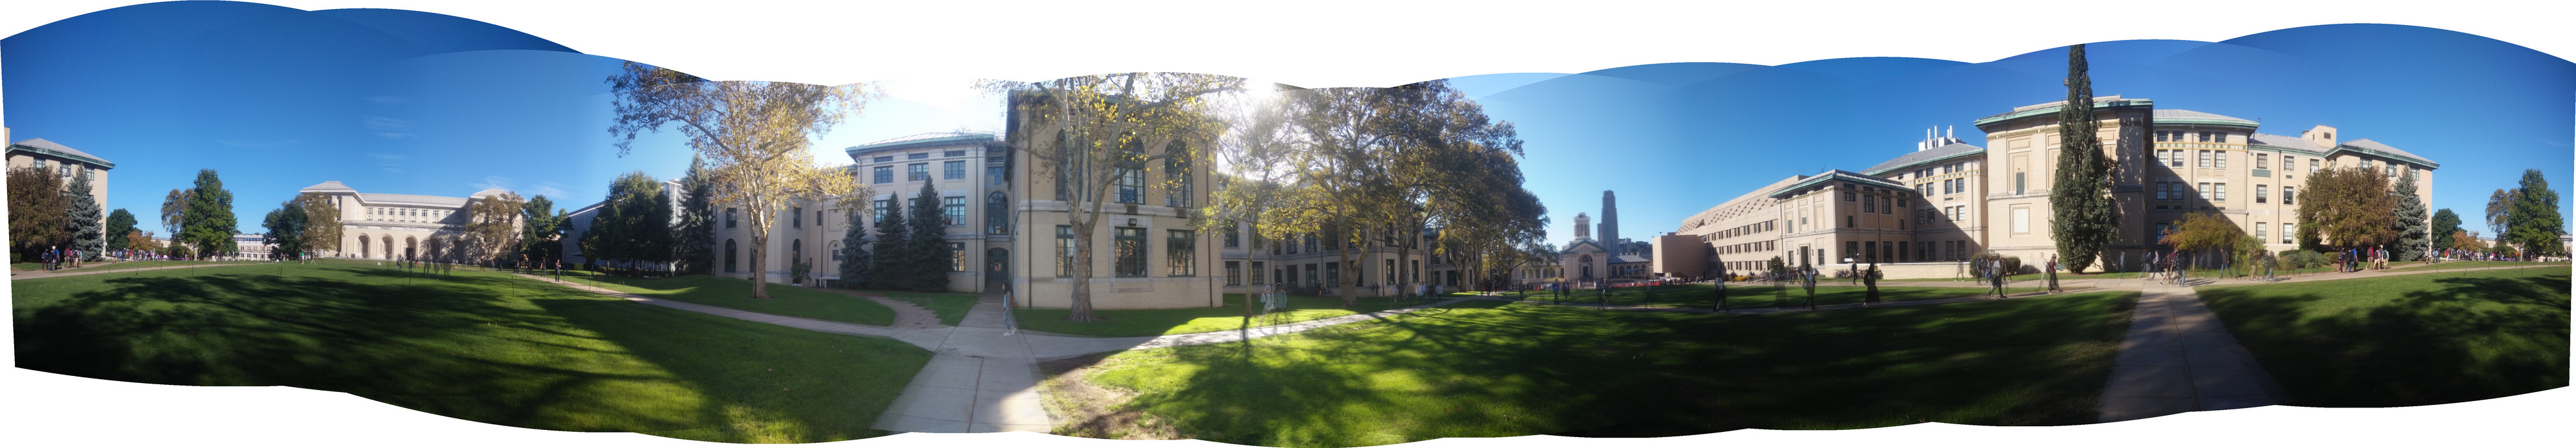
\includegraphics[width=\textwidth]{res/after-ba.jpg}
  \caption{After Bundle Adjustment}
\end{figure}

I noticed that in some hard cases, bundle adjustment cannot converge to a good result.
This is usually due to false matches or low-quality matches between images.
\cite{panoramic-sift} suggests incrementally adding images to the bundle adjuster,
which sounds reasonable but I don't have time to implement that for now.
Also, I think it'll also help to reject some matches if it is inconsistent with
the current bundle.

\subsection{Straightening}
As suggested by \cite{panoramic-sift}, the result of bundle adjustment
can have wavy effect, due to the unknown tilt angle.
By assuming all cameras have their $X$ vectors lying on the same plane,
we can estimate a $Y$ vector perpendicular to that plane
to account for the tilt and fix the wavy effect. This part
is implemented in \verb|stitch/camera.cc|.

See the following two images and notice the straight line on the grass
is corrected (it is actually a circle in the center of a soccer field).
\begin{figure}[H]
  \centering
  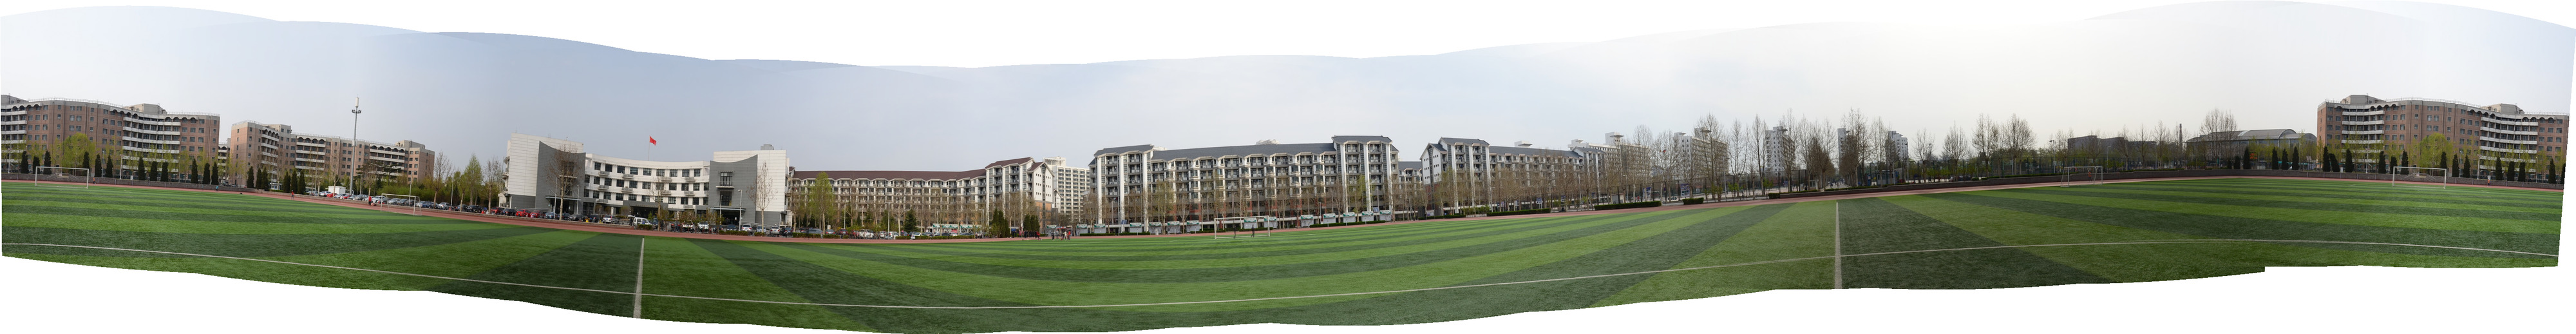
\includegraphics[width=\textwidth]{res/wavy.jpg}
  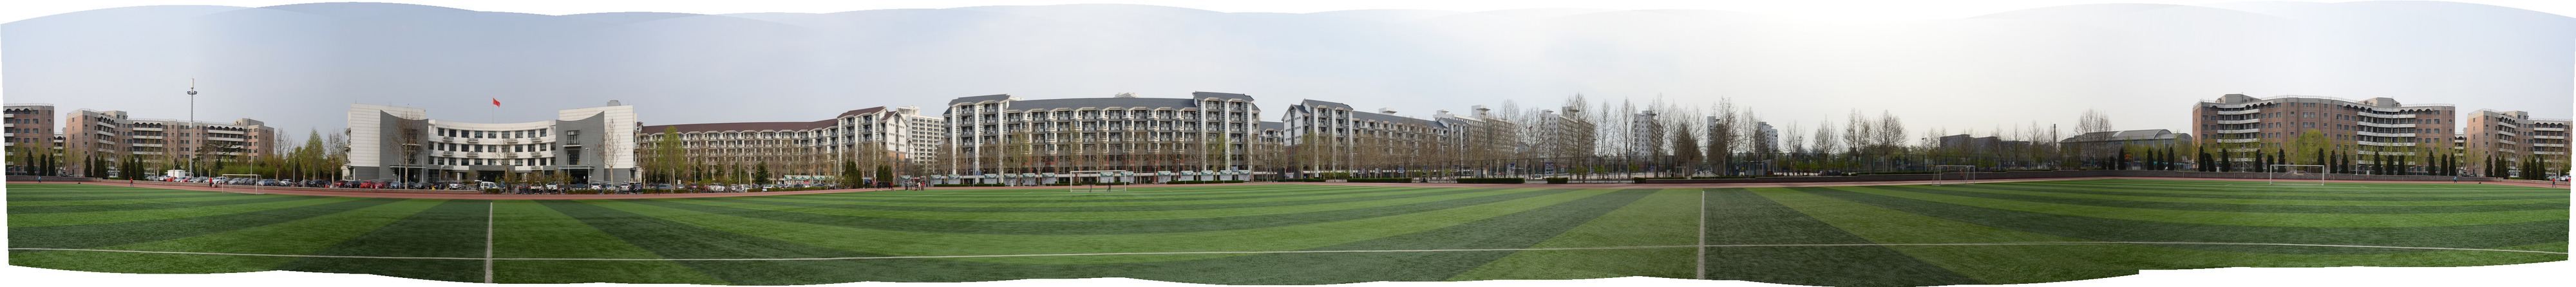
\includegraphics[width=\textwidth]{res/unwavy.jpg}
  \caption{Unstraightened and straightened result\label{fig:general-straighten}}
\end{figure}



\section{Blending}
The size of the final result is determined after having all the transformations.
And the pixel value in the result image is calculated
by an inverse transformation and bilinear interpolation with nearby pixels,
in order to reduce alias effect.

For overlapped regions, the distance from the
overlapped pixel to each image center is used to calculate
a weighted sum of the pixel value.
I only used the distance along the $x$ axis to calculate the weight,
to get better result in panoramic image.
The result is almost seamless. Compare \figref{unbend-persp} and \figref{general-straighten}
to see the effect of blending.

\section{Cropping}
When the option \verb|CROP = 1| is set,
the program simply manage to find a rectangular with largest area within the original result.

A $ O(n \times m)$ algorithm is used, where $ n, m$ is the height and width of the original result.
The algorithm works like this:

For each row $i$, the update
\begin{flalign*}
  h[j] &= \begin{cases}0,& if\ i = 0\ or\ A[i][j]\ is\ outside\ the\ area\\ h[j] + 1,& otherwise\end{cases}\\
  r[j] &= \max\{ k \in [0, m) \cap \mathbf{N}: h[t] \ge h[j], \forall j \le t \le k\} \\
  l[j]  &= \min\{ k \in [0, m) \cap \mathbf{N} : h[t] \ge h[j], \forall k \le t \le j\}\\
\end{flalign*} for every $ j \in [0, n) $ can be done in amortized $ O(1)$ time, and the corresponding area is $ (r[j] - l[j] + 1) \times h[j]$.
After the iteration, the rectangular $[i - h[j] + 1, i] \times [l[j], r[j]] $ with maximum area is our result.

The cropped final result is shown in \figref{cropped}
\begin{figure}[H]
  \centering
  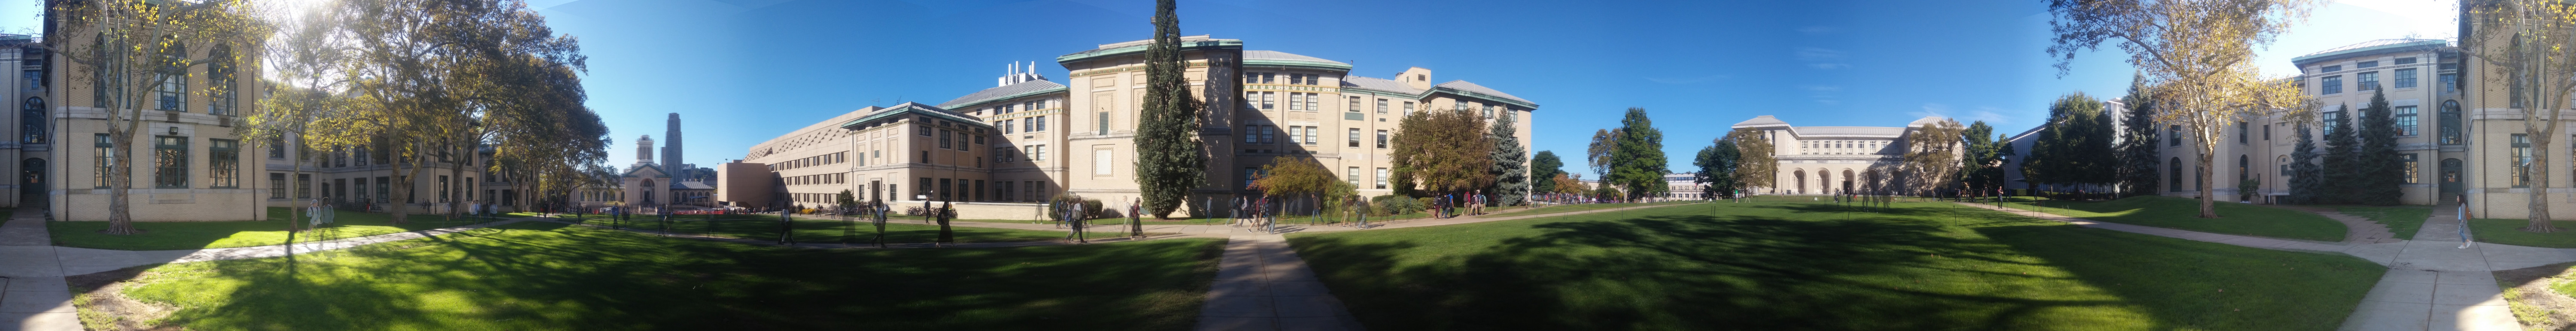
\includegraphics[width=\textwidth]{res/results/CMU1.jpg}
  \caption{Cropped Result\label{fig:cropped}}
\end{figure}

